\section{方法}

\begin{figure}[tb]
\centering
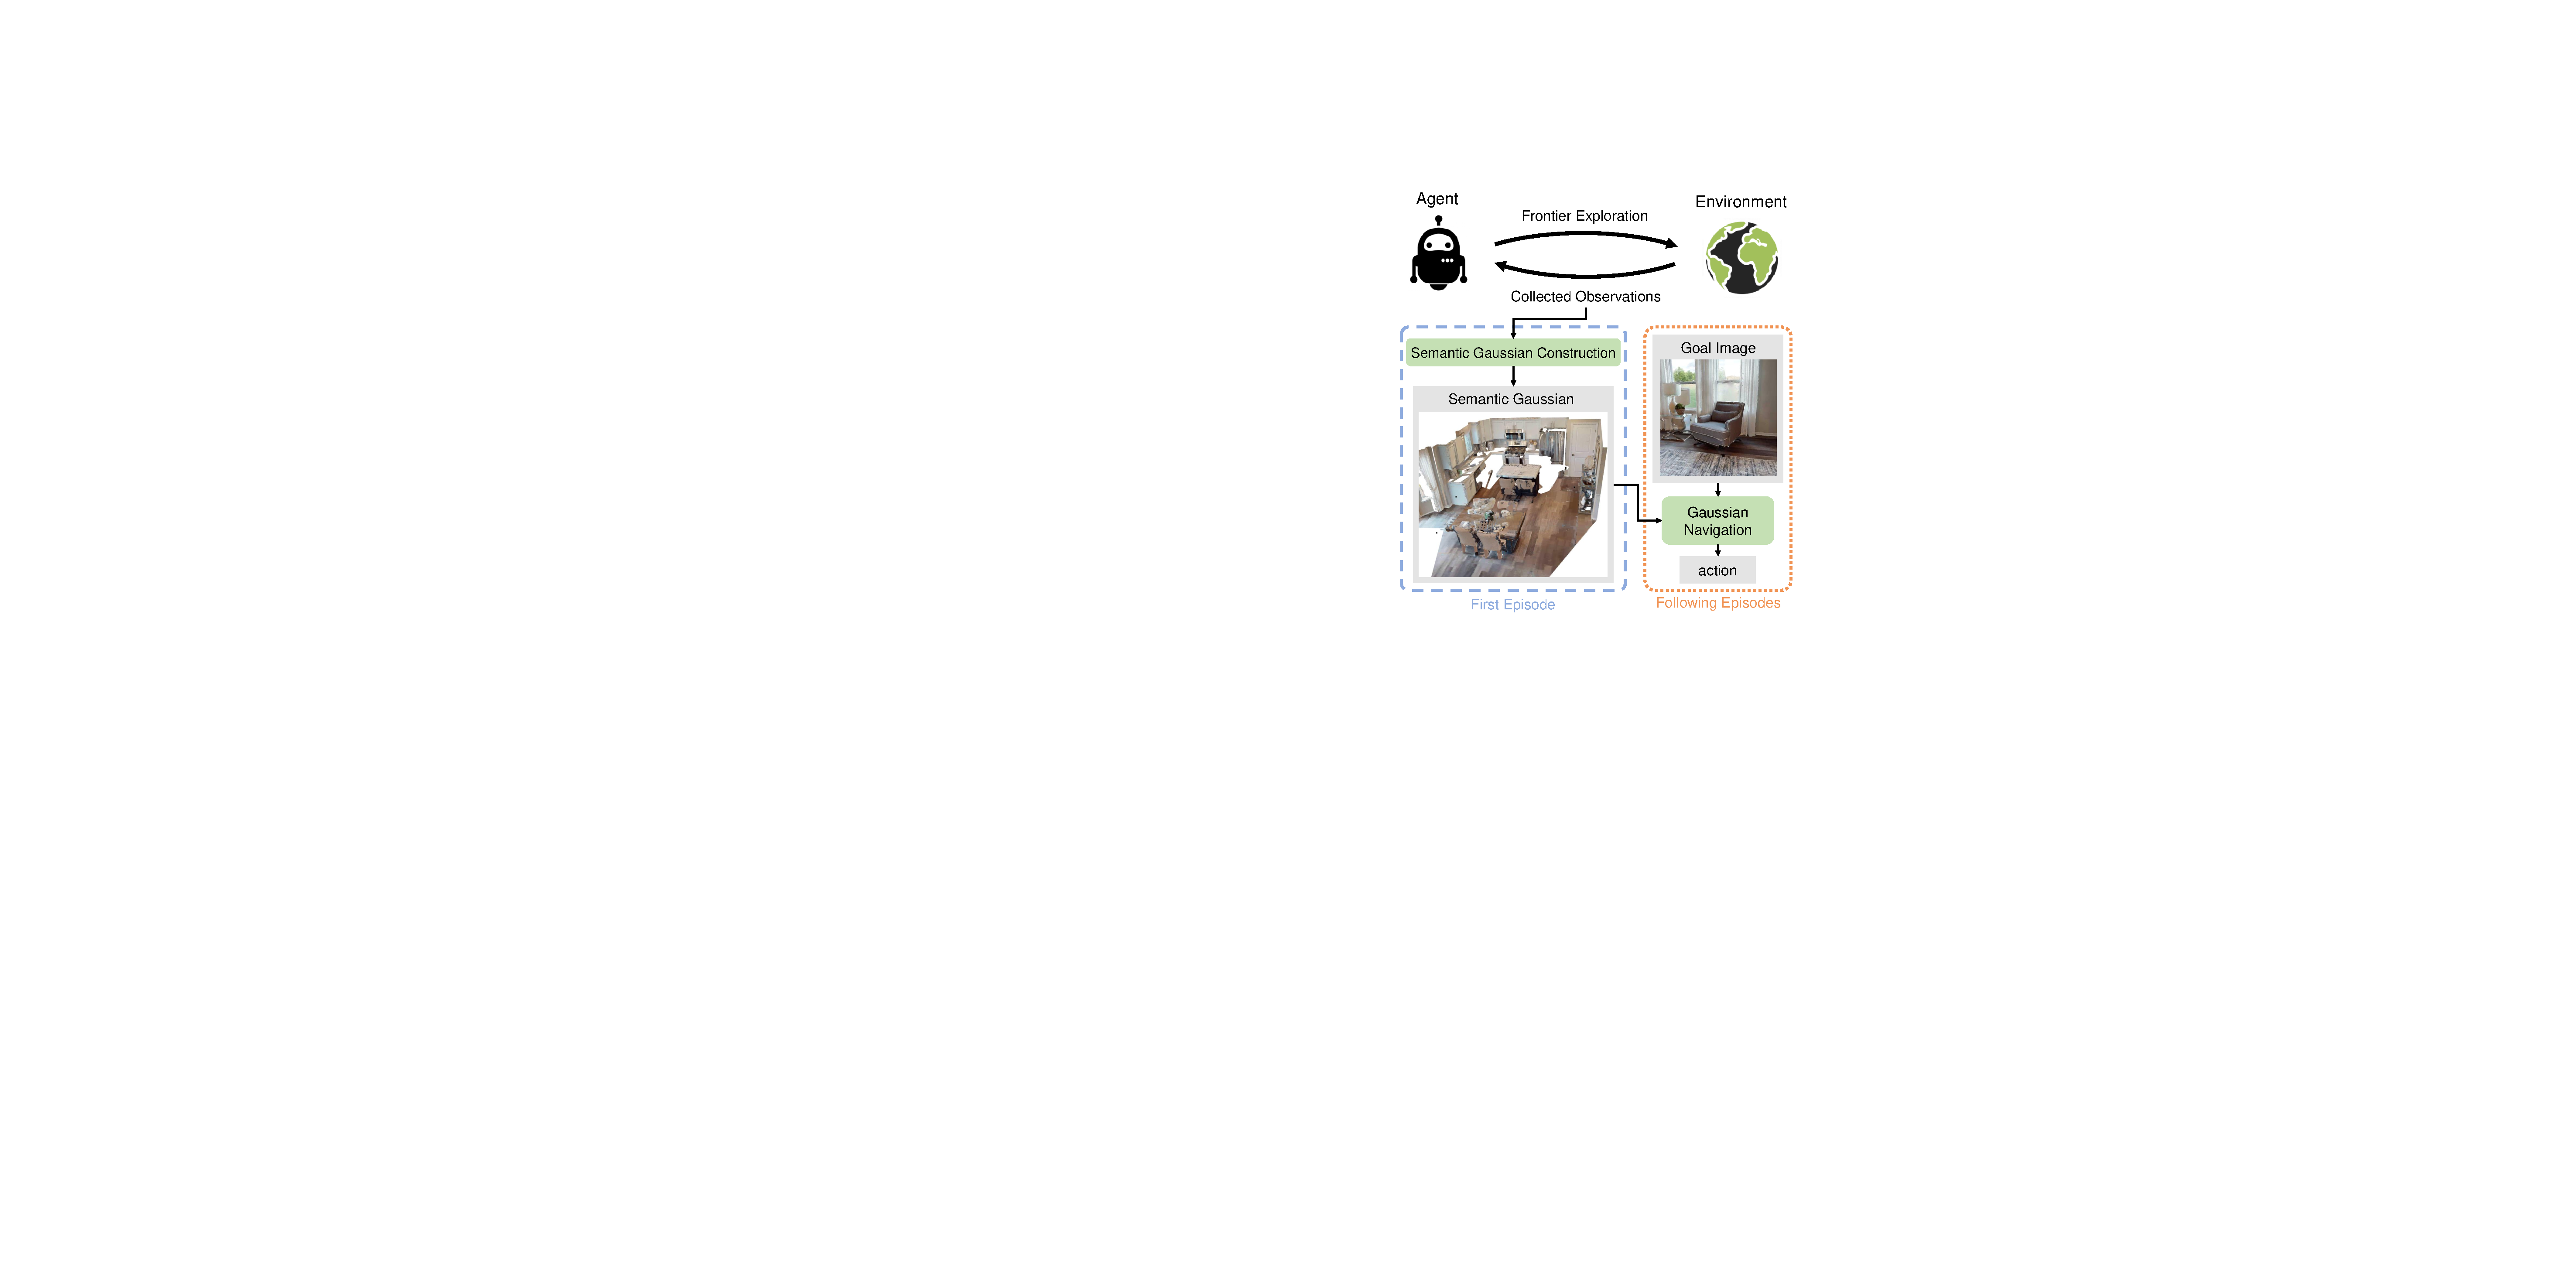
\includegraphics[width=0.95\linewidth]{pics/overview.pdf}
\caption{框架总览。在场景的第一个回合中，智能体使用前沿探索收集未知环境的观测数据，构建语义高斯地图。在后续回合中，高斯导航模块利用预构建的语义高斯地图定位目标物体并引导智能体向其移动。}
\vspace{-6pt}
\label{fig:framework_overview}
\end{figure}

\begin{figure}[tb]
\centering
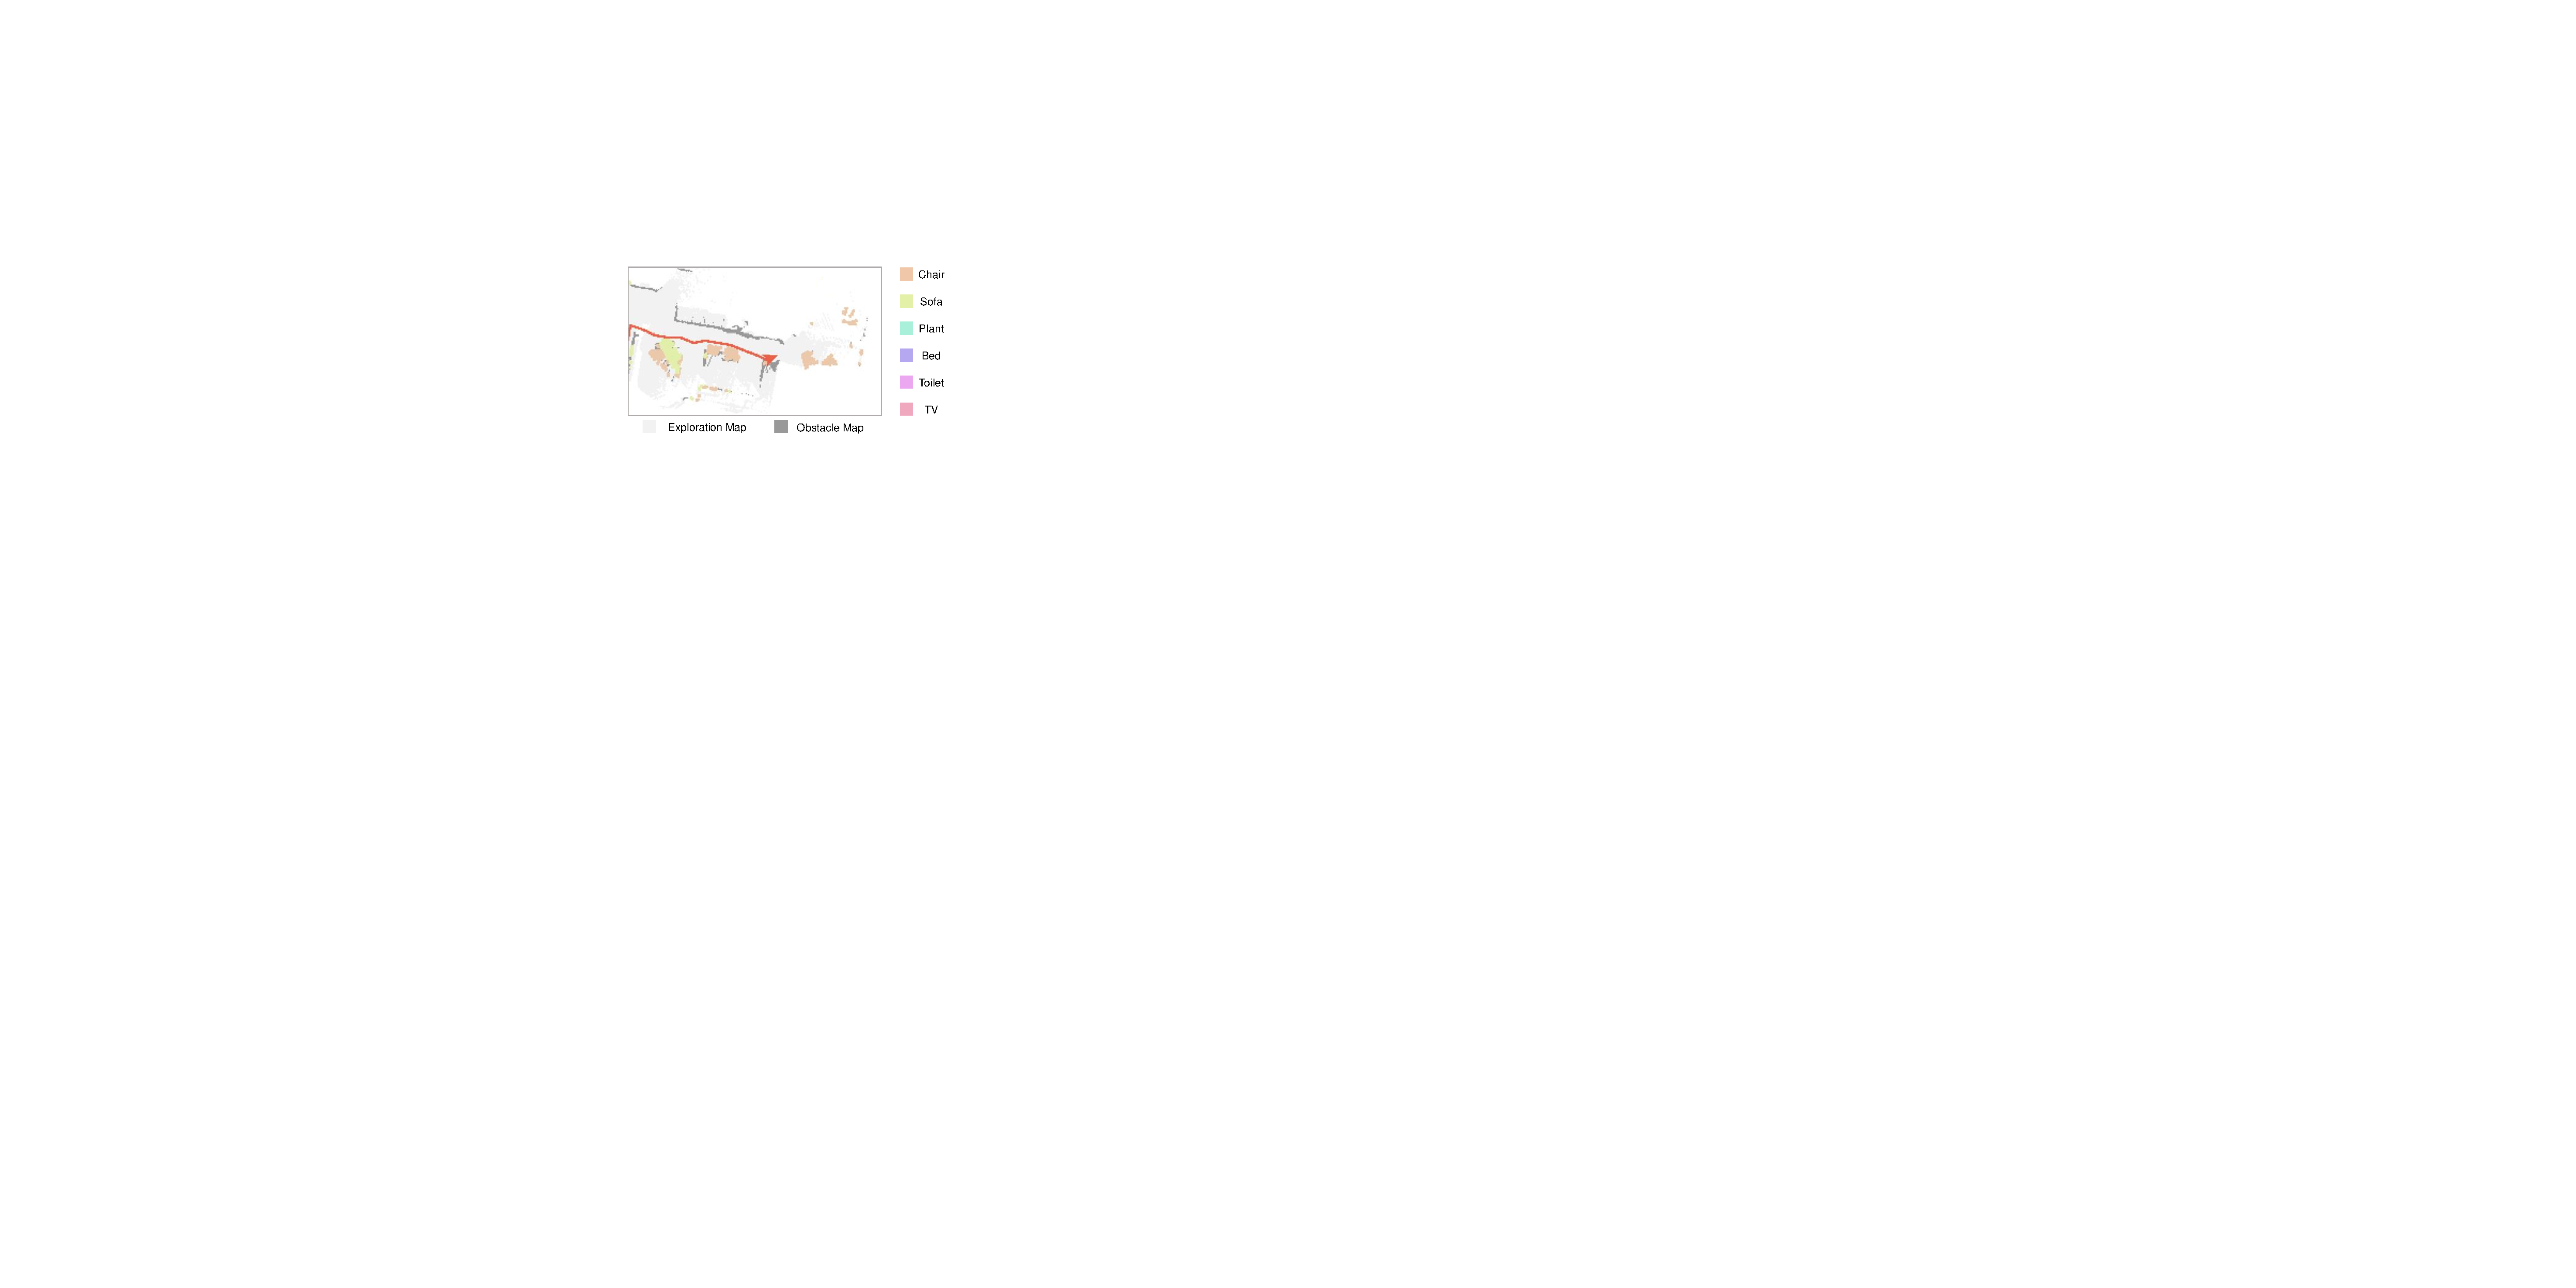
\includegraphics[width=0.98\linewidth]{pics/map.pdf}
\caption{探索地图与障碍物地图。}
\vspace{-16pt}
\label{fig:exp_obs_map}
\end{figure}

% \begin{figure*}
%   \centering
%   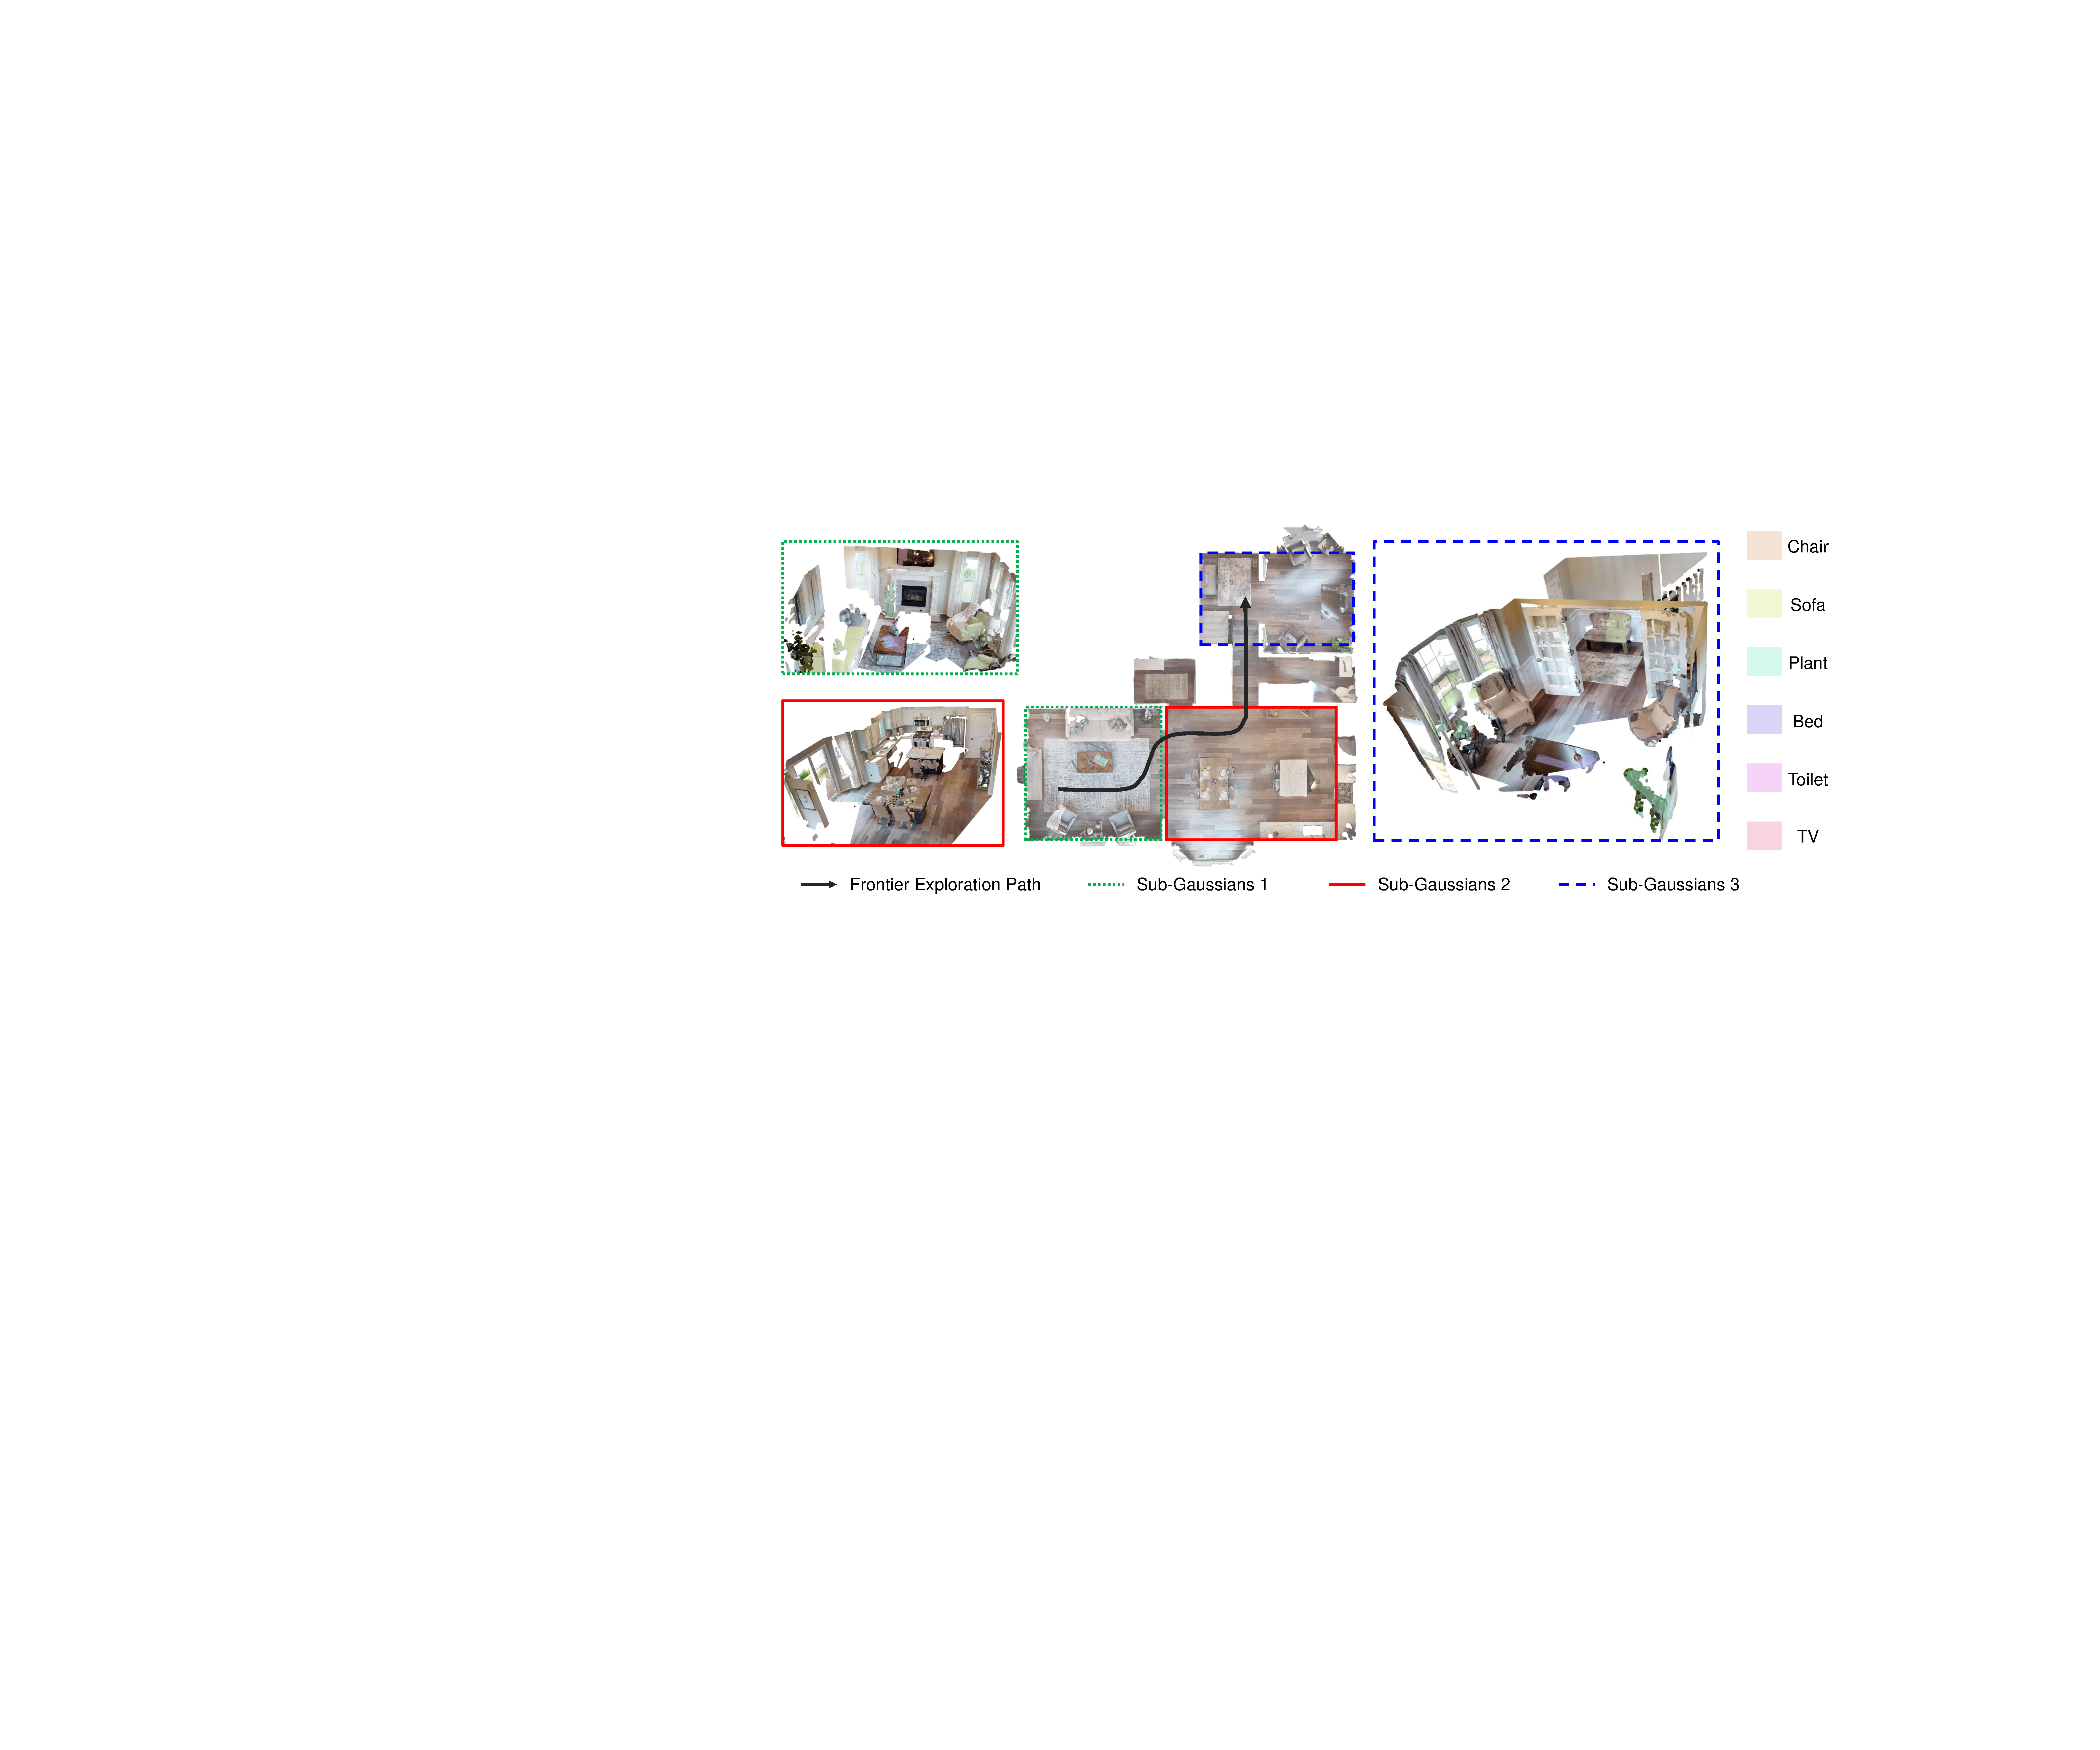
\includegraphics[width=0.95\linewidth]{pics/sub-gauss.pdf}
%   \caption{子高斯划分示意图。在未知环境中初始化时，智能体首先采用前沿探索策略探索环境。随后，智能体将收集到的观测数据划分为不同子集以构建子高斯，为后续的语义高斯构建做准备。
%   }
%   \vspace{-16pt}
%   \label{fig:sub-gauss}
% \end{figure*}


\subsection{概述}

在实例图像目标导航(IIN)任务中，新回合$e$开始时，智能体将获得一张包含指定物体实例$O_g$的目标图像$I_g$。智能体的目标是在环境中导航至该目标实例$O_g$。在每个时间步$t$，智能体获取的观测数据包括RGB图像$I_t$、深度图像$D_t$和传感器位姿读数$P_t$。智能体必须利用这些信息决定并执行动作$a_t$。当智能体调用停止动作时，只有当它处于目标物体的一定范围内，该回合才被判定为成功。

为完成IIN任务，我们提出了一个模块化框架——面向视觉导航的三维高斯泼溅技术(GaussNav)，如\Cref{fig:framework_overview}所示。在新环境中，我们提出的框架将实例图像目标导航任务分解为三个阶段：前沿探索、语义高斯构建（如\Cref{fig:gauss_construct}所示）和高斯导航（如\Cref{fig:main}所示）。首先，在未知环境的第一个回合中，智能体采用前沿探索策略探索环境并收集观测数据。随后，我们使用提出的语义高斯地图重建场景。在后续回合中，智能体利用语义高斯地图定位目标图像中描绘的物体实例$o$并导航至该位置。这一过程有效地将IIN任务转化为更易处理的点目标导航(PointGoal Navigation)任务。

\subsection{前沿探索}

在未探索环境的第一个回合中，智能体同时维护两种地图：探索地图和障碍物地图，如\Cref{fig:exp_obs_map}所示。探索地图描绘了环境中已被探索的区域，而障碍物地图则标记了场景中的障碍物。通过检测探索地图的轮廓并排除障碍物地图中的区域，智能体将最近的前沿点设置为航点以推进探索。基于前沿的探索策略是机器人学和自主导航领域中一种成熟的方法\cite{yamauchi1997frontier, holz2010evaluating}。它涉及识别环境中已探索区域与未探索区域之间的边界，即前沿。然后，智能体选择最近的可到达前沿点作为下一个探索目标。这一决策基于到前沿的距离、路径的可通行性以及探索该前沿可能获得的信息增益\cite{julia2012comparison}。通过迭代探索最近的前沿点，智能体能够高效地覆盖整个环境，同时避开障碍物和已探索区域。通过应用这种基于前沿的探索策略，智能体收集到了整个环境的观测数据。

\subsection{语义高斯构建}

我们的语义高斯地图由一组高斯表示，每个高斯由最少9个参数表征：RGB颜色向量三元组$\mathbf{c}$、质心坐标三元组$\bm{\mu} \in \mathbb{R}^3$、半径标量$r$、不透明度标量$o \in [0,1]$以及类别标签标量$l$。与原始三维高斯泼溅(3DGS)\cite{kerbl3Dgaussians}不同，我们简化了高斯的表示，仅使用视角无关的颜色并将高斯约束为各向同性。这种简化在降低内存需求的同时提高了计算效率。为全面理解三维高斯泼溅技术，我们强烈建议读者参考原始论文\cite{kerbl3Dgaussians}。我们的语义高斯构建过程可描述为一个包含两个交替步骤的迭代过程：高斯稠密化和语义高斯更新，如\Cref{fig:gauss_construct}所示。高斯稠密化在每个新帧到来时向语义高斯地图中添加新的高斯，而语义高斯更新则通过可微渲染优化每个高斯的参数。

\textit{可微渲染。} 三维高斯泼溅(3DGS)\cite{kerbl3Dgaussians}按如下方式渲染RGB图像：给定一组三维高斯和相机位姿，首先将所有高斯按从前到后的顺序排序。然后，通过在像素空间中按顺序对每个高斯的二维投影进行alpha合成，可以高效地渲染出RGB图像。像素${\bf p} = (u,v)$的渲染颜色可表示为：
\begin{equation}
\hat{I}(\mathbf{p}) = \sum_{i=1}^{n} \mathbf{c}_i f_i(\mathbf{p}) \prod_{j=1}^{i-1} (1 - f_j(\mathbf{p})),
\end{equation}
其中$f_i(\bf{p})$的计算方式如下：
\begin{align}
    f(\mathbf{x}) = o \exp\left(-\frac{\|\mathbf{x} - \boldsymbol{\mu}\|^2}{2r^2}\right).\label{eq:gauss}
\end{align}
$\boldsymbol{\mu}$和$r$是像素空间中投影后的二维高斯参数：
\begin{equation}
    \boldsymbol{\mu}^{\textrm{2D}} = K \frac{E_t \boldsymbol{\mu}}{d}, \;\;\;\;\;\;
r^{\textrm{2D}} = \frac{f r}{d}, %
\quad \text{其中} \quad d = (E_t \boldsymbol{\mu})_z.
\end{equation}
这里，$K$是相机内参矩阵，$E_t$是编码$t$时刻相机旋转和平移的外参矩阵，$f$是已知的焦距，$d$是第$i$个高斯相对于相机坐标系的深度。

\textbf{渲染。} 与三维高斯泼溅(3DGS)\cite{kerbl3Dgaussians}不同，我们可微地渲染深度图和轮廓图，这决定了可见性，并将用于后续的高斯稠密化和更新。像素$\mathbf{p}$处的深度$\hat{D}$和轮廓$\hat{S}$的渲染方式如下：
\begin{equation}
    \hat{D}(\mathbf{p}) = \sum_{i=1}^{n} d_i f_i(\mathbf{p}) \prod_{j=1}^{i-1} (1 - f_j(\mathbf{p})), 
\end{equation}
\begin{equation}
    \hat{S}(\mathbf{p}) = \sum_{i=1}^{n} f_i(\mathbf{p}) \prod_{j=1}^{i-1} (1 - f_j(\mathbf{p})).
\end{equation}
在此基础上，我们还渲染语义分割结果：
\begin{equation}
    \hat{C}(\mathbf{p}) = \sum_{i=1}^{n} l_i f_i(\mathbf{p}) \prod_{j=1}^{i-1} (1 - f_j(\mathbf{p})).
\end{equation}

\textbf{语义分割。} 如\Cref{fig:gauss_construct}所示，智能体的RGB观测$I_t$通过Mask-RCNN\cite{he2017mask}被分割为$C_t$。分割结果将用于在高斯稠密化阶段初始化新的高斯，并在语义高斯更新阶段监督高斯参数的优化。

\textbf{高斯稠密化。} 高斯稠密化通过将$t-1$时刻的高斯在位置$P_t$处的渲染结果与真实值进行比较来执行。该过程在先前的高斯无法表示新观测中的场景区域时添加新的高斯。遵循Keetha等人\cite{keetha2023splatam}的方法，我们基于稠密化掩码确定哪些像素需要进行稠密化：
\begin{equation}
\small
M(\textbf{p}) = \Bigl(\hat{S}(\textbf{p}) < 0.5\Bigr) + \Bigl( D(\textbf{p}) < \hat{D}(\textbf{p}) \Bigr) \Bigl(\textrm{L}_1\bigl(\hat{D}(\textbf{p})\bigr) > 50 \textrm{MDE} \Bigr),
\end{equation}
其中第一项表示语义高斯不够稠密的区域，第二项表示真实深度在预测深度之前且深度误差大于50倍中值深度误差(MDE)的区域。

\textbf{语义高斯更新。} 在对当前语义高斯地图进行稠密化后，我们根据位姿和观测数据更新高斯的参数。这通过可微渲染和基于梯度的优化来实现，等价于将辐射场拟合到已知位姿图像的"经典"问题。具体而言，我们通过最小化RGB、深度和分割误差来更新高斯的参数。

\begin{figure}[tb]
\centering
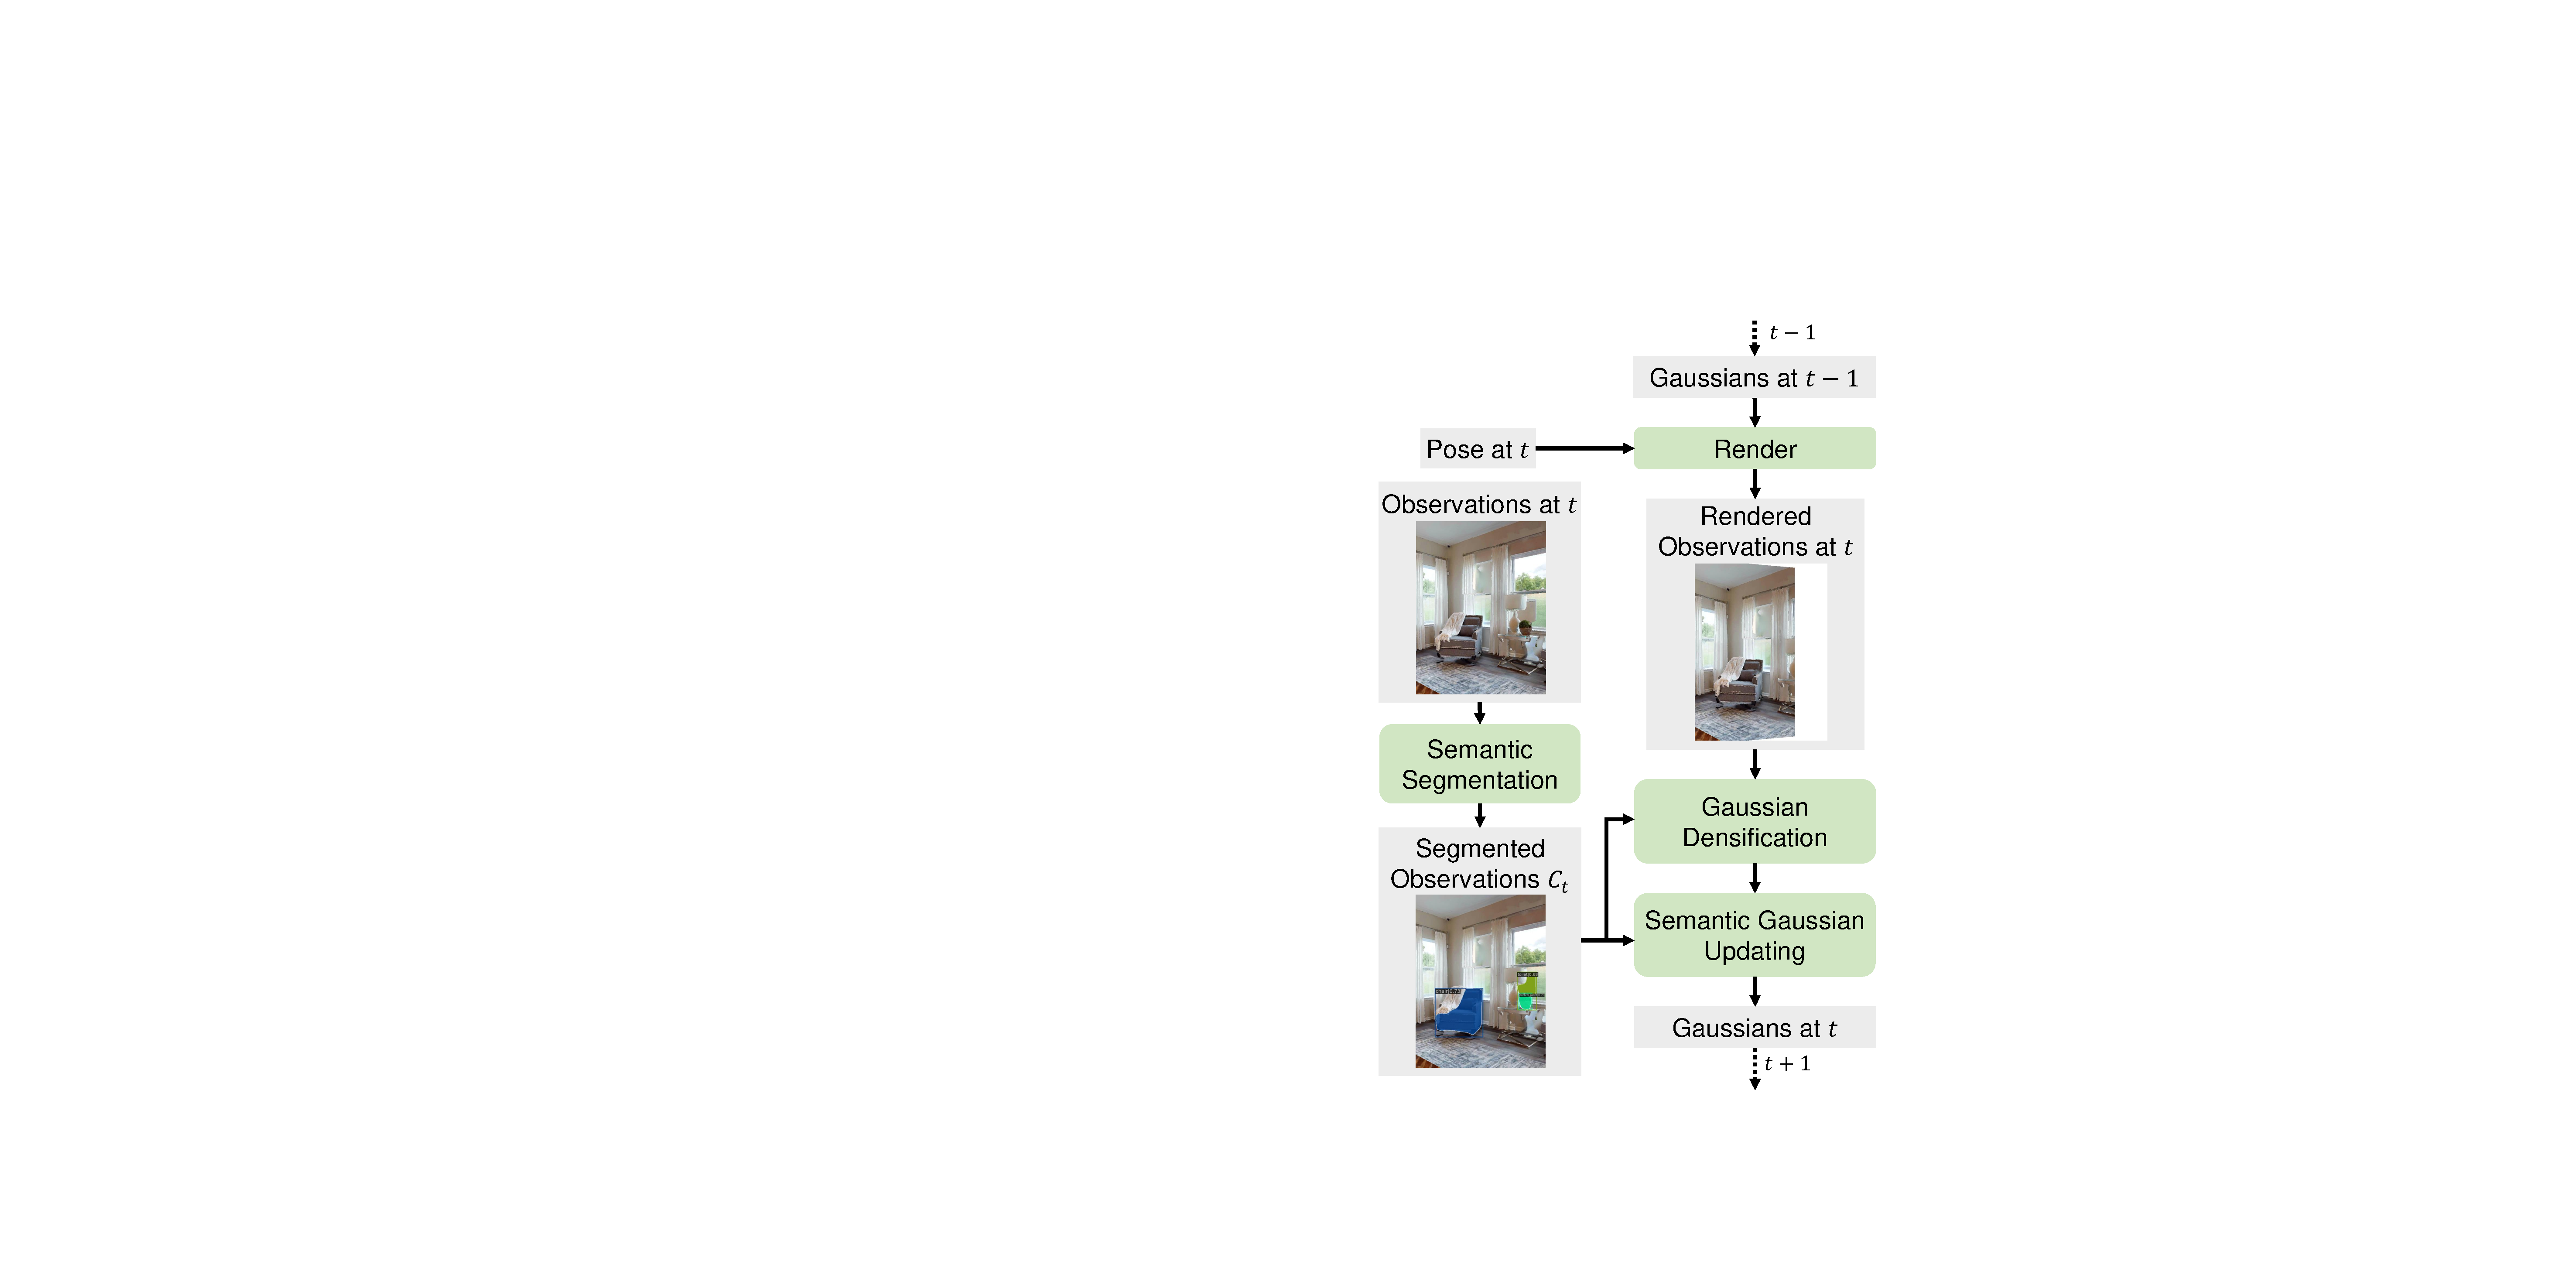
\includegraphics[width=0.8\linewidth]{pics/gauss_cons.pdf}
\caption{语义高斯构建示意图。在时间步$t$，流水线通过稠密化和更新步骤优化$t-1$时刻的高斯，这涉及将渲染的RGB和深度图像与当前输入的训练视图进行比较。同时，使用分割图像为稠密化后的高斯分配语义标签。最后，通过可微渲染对高斯进行精调。}
\label{fig:gauss_construct}
\vspace{-10pt}
\end{figure}

\begin{figure}[tb]
\centering
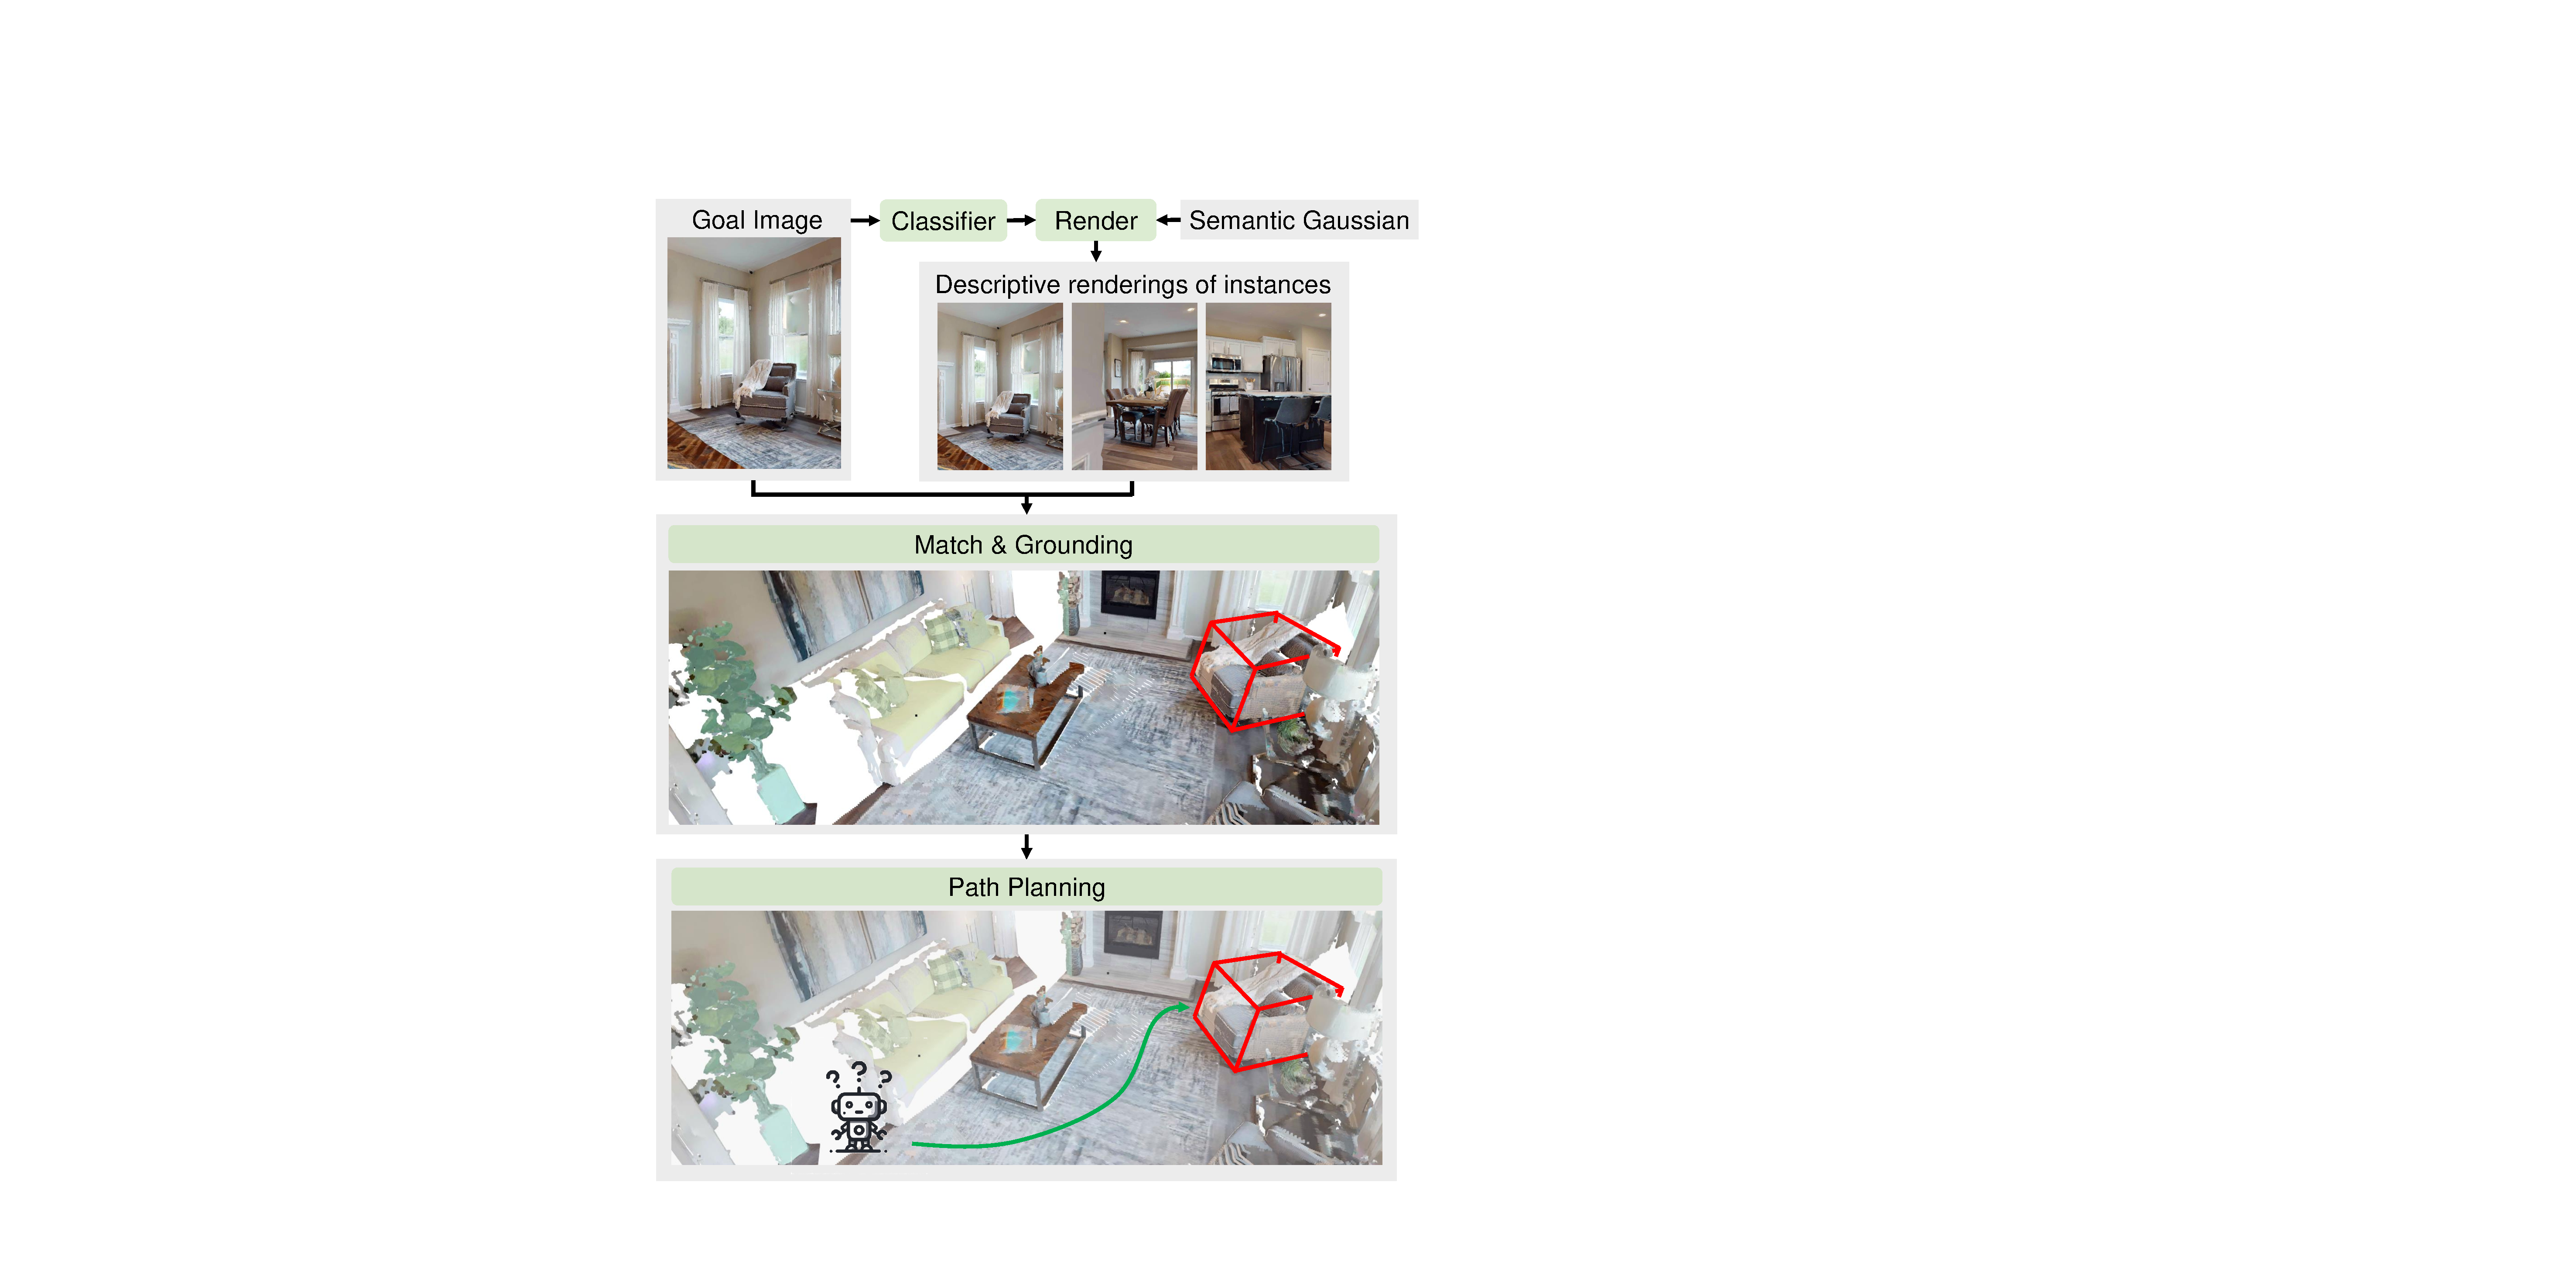
\includegraphics[width=0.9\linewidth]{pics/main.pdf}
\caption{高斯导航示意图。我们的方法首先使用预构建的语义高斯地图对目标图像进行分类。在确定预测类别后，我们围绕属于该类别的实例生成描述性图像。然后将这些图像与目标物体进行匹配，以识别并定位目标实例。利用地图和确定的目标，智能体采用路径规划算法计算动作序列。}
\label{fig:main}
\vspace{-10pt}
\end{figure}

\subsection{高斯导航}

为利用构建好的语义高斯地图进行导航，我们提出了高斯导航方法，如\Cref{fig:main}所示。我们首先对目标图像$I_g$进行分类，预测当前目标的语义标签$\hat{l}_g$，例如\Cref{fig:main}中的"椅子"。然后使用该语义标签查询相关的高斯。对于每个属于同一类别的相关物体实例，我们渲染描述性图像。将这些渲染结果与目标图像进行比较以定位目标物体，预测其位置$\hat{P}_g$。最后，路径规划模块生成可行路径并确定智能体的动作。

% 一旦语义高斯地图构建完成且智能体的初始位姿已知，将IIN转化为点目标导航需要：1. 将语义高斯地图转换为可用于路径规划的地图形式，即三维体素$M_{3D}$或二维鸟瞰图栅格$M_{2D}$；2. 预测目标物体实例的位置$\hat{P}_g$。因此，我们首先将语义高斯地图转换为点云，其中每个高斯被简化为点云表示中的一个点。然后将点云体素化为三维体素$M_{3D}$，再将三维体素$M_{3D}$投影为二维鸟瞰图栅格$M_{2D}$。通过在预构建的语义高斯地图$G_s$中与目标图像$I_g$进行分类和匹配，我们可以定位目标物体的位置$\hat{P}_g$，如\Cref{fig:main}所示。给定起始位姿$P_0$、预测的目标物体位置$\hat{P}_g$和栅格地图$M_{2D}$，我们可以轻松使用快速行进法(FMM)\footnote{\url{https://pythonhosted.org/scikit-fmm/}}计算最短路径和对应的动作$a_t$。

\textbf{分类器。} 在IIN任务中，智能体接收一张描绘目标物体的图像$I_g$。然而，由于搜索空间巨大，将该图像与整个场景中所有可导航点的渲染结果进行比较会极其耗时。因此，借助我们的语义高斯地图$G_s$，我们只需搜索与目标物体对应类别的实例。为此，我们首先将目标图像$I_g$分类为目标类别标签$\hat{l}_g$。我们使用HM3D-SEM\cite{yadav2023habitat}训练集上的目标图像对在ImageNet\cite{5206848}上预训练的图像分类模型ResNet50\cite{He2015}进行微调。

% 相比之下，为了在现实世界中获得更好的泛化能力，无需对模型进行微调。

\textbf{匹配与定位。} 利用预测的目标物体标签$\hat{l}_g$，我们识别出所有具有相同类别标签的候选物体。对于每个候选实例，我们通过从多个视角渲染物体来生成一组描述性图像，以捕捉其特征。具体而言，对于包含潜在候选物体的一个训练视图，我们通过新视角合成(NVS)将其增强为$n_v$个视图。我们将训练视图的相机到世界坐标系的变换记为$\text{c2w}$，并将潜在目标物体在相机坐标系中的平移向量记为$\mathbf{t}^{o}_{c}$。我们使用\textit{前向}、\textit{右向}和\textit{上向}向量定义物体到世界坐标系的旋转矩阵。\textit{前向}方向是从训练视图到潜在目标物体的向量，即$\mathbf{t}^{o}_{c}$。\textit{上向}方向是向量$[0,\,-1,\,0]$，\textit{右向}向量与\textit{前向}和\textit{上向}向量都正交，与\textit{右向}、\textit{上向}和\textit{前向}向量共同构成右手坐标系。物体到世界坐标系的平移向量为：
    \begin{equation}
        \mathbf{t}^{o}_{w} = \text{c2w} \times \mathbf{t}^{o}_{c}.
        \label{equ:NVS0}
\end{equation}
旋转矩阵和平移向量共同构成了从物体到世界坐标系的刚性变换矩阵$\text{o2w}$。

我们将绕$y$轴和$x$轴的旋转矩阵分别定义为$\mathbf{R}_y(\theta)$和$\mathbf{R}_x(\theta)$，分别表示在水平和垂直方向上绕物体旋转$\theta$角形成的新视角。因此，水平方向上新视角的相机到世界坐标系变换为：
\begin{equation}
    \text{c2w}_h(\theta) = \text{o2w} \times \mathbf{R}_y(\theta) \times \text{w2o} \times \text{c2w},
    \label{equ:NVS1}
\end{equation}
垂直方向上为：
\begin{equation}
    \text{c2w}_v(\theta) = \text{o2w} \times \mathbf{R}_x(\theta) \times \text{w2o} \times \text{c2w}.
    \label{equ:NVS2}
\end{equation}
在实验中，当$n_v=1$时，我们不执行新视角合成；当$n_v=3$时，我们在$\theta = \pm15^\circ$（水平和垂直方向）执行新视角合成；当$n_v=5$时，我们使用$\theta = \pm15^\circ$和$\pm30^\circ$。

新视角合成后，原始训练视图得到增强。第$i$个物体实例的增强渲染集记为$S_i$。设$n$为与目标物体同类别观测到的实例数，则$S$的全集可表示为：
\begin{equation}
    S = \{S_1, S_2, \ldots, S_n\}  \quad \text{其中} \quad i=1,2,\ldots,n.
\end{equation}
为从这些候选物体中区分出目标物体，我们将问题表述为：
\begin{equation}
\begin{split}
      i_{\text{max}} = arg\max \{ \max_{s \in S_1} \Omega (s), \max_{s \in S_2} \Omega (s), \ldots, \max_{s \in S_n} \Omega (s) \} \\
      \text{其中} \quad i=1,2,\ldots,n,
    \label{eq:match}  
\end{split}
\end{equation}
其中$\Omega (\cdot)$定义为渲染图与目标图像$I_g$之间匹配的关键点数量。具体而言，对于第$i$个物体实例的渲染图$s \in S_i$和目标图像$I_g$，我们使用DISK\cite{tyszkiewicz2020disk}提取关键点的像素坐标$(x, y)$及其关联的特征描述子$V_t$。即：
\begin{equation}
(K_t, V_t) = \text{DISK}(s), \quad (K_g, V_g) = \text{DISK}(I_g).
\label{eq:feature1}
\end{equation}
随后，使用LightGlue\cite{lindenberger2023lightglue}计算匹配对$(\hat{K_t}, \hat{K_g})$。特征匹配过程可表述为：
\begin{equation}
(\hat{K_t}, \hat{K_g}) = \text{LightGlue}((K_t, V_t), (K_g, V_g)).
\label{eq:matching}
\end{equation}
因此，匹配点的数量，即$\hat{K_t}$或$\hat{K_g}$的长度，记为$\Omega$。渲染图像产生最多匹配关键点的候选物体被选为目标物体，如\Cref{eq:match}所示。

当物体实例被选中后，我们在语义高斯地图中定位该物体。由于语义分割误差会导致离群点的存在，我们对地图上的实例进行聚类。具体而言，我们使用基于密度的空间聚类算法(DBSCAN)\footnote{\url{https://scikit-learn.org/stable/modules/generated/sklearn.cluster.DBSCAN.html}}，该算法将紧密聚集的点归为一类，将低密度区域中孤立的点标记为离群点。通过精确确定所选物体实例的位置，我们可以轻松地将IIN任务转化为点目标任务。

\textbf{路径规划。} 语义高斯地图并非为路径规划设计。我们首先将语义高斯地图转换为点云，其中每个高斯被简化为点云表示中的一个点。然后将点云体素化为三维体素$M_{3D}$，再将三维体素$M_{3D}$投影为二维鸟瞰图栅格$M_{2D}$。这里，我们使用语义高斯地图的二维投影而非预探索阶段使用的二维几何地图，以保持整个流水线表示的一致性。我们的语义高斯地图使用从深度图像导出的点云初始化高斯，并且在优化阶段不修剪任何高斯。因此，语义高斯地图的二维投影与二维几何地图在本质上是等价的。

给定二维鸟瞰图栅格地图$M_{2D}$，以及智能体的起始位置和目标位置，我们可以使用快速行进法(FMM)高效生成最短距离场。该场中的每个点都包含从起点到该点所需的最小距离。我们提取该距离场中落在智能体操作范围内的相关子集。随后，从该子集中选择一个航点，确保它不与任何障碍物相交且位于距离场的局部最小值处。根据所选航点，智能体可以根据当前状态的角度和距离轻松计算出动作。智能体迭代执行上述过程生成动作序列，直到到达目的地。